\documentclass[12pt,spanish, singlespacing,]{MastersDoctoralThesis}
\usepackage[utf8]{inputenc} 
\usepackage[T1]{fontenc} 
\usepackage[none]{hyphenat}
\usepackage{palatino} 
\usepackage{acronym}
\spacing{1.5}
\usepackage[nomain]{glossaries}
%\usepackage[backend=bibtex,style=authoryear,natbib=true]{biblatex}
%\addbibresource{main.bib}
\usepackage[autostyle=true]{csquotes}

\usepackage{afterpage}
\newcommand\blankpage{%
    \null
    \thispagestyle{empty}%
    \addtocounter{page}{0}%
    \newpage}
    
\usepackage{listings}
\renewcommand{\lstlistingname}{Código}
\renewcommand\lstlistlistingname{Índice de Código}

\usepackage{float}
\usepackage{url}
\usepackage{algorithm}
\usepackage{algpseudocode}
\usepackage{amsfonts}
\usepackage{graphicx}
\usepackage{tikz}
\usetikzlibrary{arrows.meta,positioning,shapes.geometric}
\makeatletter
\g@addto@macro{\UrlBreaks}{\UrlOrds}
\makeatother                                                  

\thesistitle{}
\supervisor{Cesar Jesus Lara Avila} 
\examiner{} 
\degree{} 
\author{Luis Alberto De la cruz Mantilla} 
\subject{}
\keywords{} 
\university{\href{http://www.uni.edu.pe/}{Universidad Nacional de Ingenier\'ia}} 
\department{\href{http://fc.uni.edu.pe/fc/index.php/escuelas/ciencia-de-la-computacion}{}} 
\faculty{\href{http://fc.uni.edu.pe/fc/}{}}
\hypersetup{pdftitle=\ttitle} 
\hypersetup{pdfauthor=\authorname}
\hypersetup{pdfkeywords=\keywordnames} 
\sloppy
\decimalpoint
\begin{document}
\frontmatter 
\pagestyle{plain} 
\begin{titlepage}
\begin{center}
%\textsc{\huge \univname}\\[0.5cm]

\begin{figure}[h]
\centering
\includegraphics[width=0.3\textwidth]{Figures/Escudo_UNI.png}
\end{figure}

\textsc{\huge \univname}\\[0.3cm]
\textsc{\Large Facultad de Ciencias}\\[0.2cm]
\textsc{\large Escuela Profesional de Ciencia de la Computaci\'on}\\[2cm]
\textsc{\LARGE \textit{Optimización Multiobjetivo de Líneas de Ensamblaje usando NSGA-II y Algoritmo Memético}}\\[2cm] 
{\Large \textbf{PROYECTO DE TESIS}}
{\huge \bfseries \ttitle}\\[2cm] 
% Thesis title
%\bigskip
%\HRule \\[0.8cm] % Horizontal line

%\begin{minipage}{1.5\textwidth}
%\begin{flushleft} \large
\bigskip
\bigskip
\large\emph{Autor:}
{\authorname}\\ 
\large\emph{Asesor:} 
{\supname} 
%\end{flushleft}
%\end{minipage}
%\\[2cm]
\\[1cm]
{\large Octubre, 2025}\\[4cm] 
 
\vfill
\end{center}
\end{titlepage}
\afterpage{\blankpage}
%\cleardoublepage
%\renewcommand{\abstractname}{Abstract}
\begin{abstract}
\addchaptertocentry{\abstractname}

Este estudio desarrolla algoritmos evolutivos multiobjetivo para programación de tareas en HFS con máquinas en paralelo. Se implementa NSGA-II y su variante memética para optimizar simultáneamente tres objetivos: minimizar makespan, balancear carga de trabajo y reducir consumo energético. La metodología considera programación realista incluyendo desgaste de máquinas y procesos de enfriamiento. Se realizó tunning multiobjetivo evaluando 1,890 configuraciones (56,700 ejecuciones) y un estudio de ablación para validar cada componente. Los resultados proporcionan 51-82 soluciones Pareto-óptimas, identificando tres soluciones representantes que priorizan cada objetivo individualmente, facilitando la selección según prioridades operativas. La comparación reveló que NSGA-II estándar es 14.0\% más rápido con calidad prácticamente idéntica. Las optimizaciones de vectorización con NumPy redujeron el tiempo de ejecución en 56.7\%, alcanzando 11.5 segundos promedio. El estudio demuestra la efectividad del algoritmo NSGA-II estándar para optimizar simultáneamente productividad, equidad de carga y consumo energético en sistemas de manufactura.

\end{abstract}
\afterpage{\blankpage}
\tableofcontents
%\afterpage{\blankpage}
\listoffigures
%\afterpage{\blankpage}
%\listoftables
%\afterpage{\blankpage}
%\listoftables 
%\lstlistoflistings
%\afterpage{\blankpage}
\newpage
\begin{center}
{\huge Índice de Acrónimos}\\[2cm]
\end{center}
\bigskip
\begin{tabular}{ l c l }
\textbf{HFS} & & Hybrid Flow Shop\\
\textbf{AE} & & Algoritmo evolutivo\\
\textbf{AG} & & Algoritmo Genético \\
\textbf{NSGA-II} & & Non-dominated Sorting Genetic Algorithm II\\
\textbf{MILP} & & Mixed Integer Linear Programming\\

\end{tabular}
\afterpage{\blankpage}

\newpage
\begin{center}
{\huge \textit{Agradecimientos}}\\[1.5cm]
\end{center}

Agradezco a mi asesor de tesis, el profesor Cesar Jesús Lara Avila, por su guía invaluable, paciencia y dedicación a lo largo de todo este proyecto. Sus orientaciones precisas y su compromiso con mi desarrollo académico han sido fundamentales para el crecimiento de este trabajo. Su disposición para ayudarme a resolver dudas, su experiencia y su interés genuino por mi progreso académico fueron una fuente constante de motivación durante este proceso. Gracias por motivarme a superar cada desafío y por brindarme la confianza necesaria para avanzar con seguridad en este trayecto académico. 

A mi familia por mostrarme su apoyo incondicional durante todo el proceso de este proyecto, especialmente durante las largas noches de trabajo, brindándome la tranquilidad necesaria para culminar con esta investigación. Su comprensión y apoyo fueron esenciales para mantener el equilibrio necesario en este periodo.

A la Facultad de Ciencias de la Universidad Nacional de Ingeniería, por permitirme utilizar la computadora del laboratorio de ciencias (conocido como "Monstrito") para ejecutar las pruebas computacionales más pesadas, como el tunning de hiperparámetros y los experimentos de comparación de operadores. El acceso a este recurso computacional fue fundamental para completar los más de 56,700 experimentos necesarios para este trabajo, permitiéndome realizar análisis exhaustivos que de otra manera no habrían sido posibles en un tiempo razonable.

A todos, gracias por acompañarme en este camino y por ser una parte fundamental en la realización de este proyecto. Su apoyo no solo enriquece mi formación académica, sino también mi crecimiento personal.

\afterpage{\blankpage}

\mainmatter 
\pagestyle{thesis}
\chapter{Introducción}
Hoy en día, la tecnología industrial avanza constantemente y la competencia global se intensifica cada vez más. Por esto, las empresas tienen que optimizar sus procesos productivos si quieren mantenerse competitivas. Las líneas de ensamblaje juegan un papel central en la fabricación, y necesitan soluciones que garanticen eficiencia, sostenibilidad y capacidad de adaptarse cuando las condiciones operativas cambian. Resolver problemas donde interactúan muchas variables simultáneamente (número de máquinas, secuencia de tareas, restricciones operativas) representa un desafío importante. Esta complejidad hace evidente que se necesitan herramientas que vayan más allá de los enfoques tradicionales, y los algoritmos evolutivos destacan como una alternativa viable.

Los algoritmos evolutivos (AE) se han posicionado como una opción potente y flexible para estos desafíos. Están inspirados en la evolución natural, lo que les permite explorar espacios de soluciones muy amplios y encontrar resultados cercanos al óptimo en problemas complejos. Esta tesis implementa algoritmos evolutivos multiobjetivo, específicamente NSGA-II y su variante memética, para optimizar simultáneamente varios aspectos al programar máquinas en líneas de ensamblaje. El objetivo es conseguir soluciones que minimicen el tiempo de producción, balanceen la carga de trabajo entre máquinas y reduzcan el consumo energético.

\section{Motivación}
Este trabajo busca implementar algoritmos evolutivos multiobjetivo que permitan encontrar programaciones óptimas para líneas de ensamblaje considerando múltiples objetivos relevantes. Optimizar los tiempos en una línea de ensamblaje ya es complicado por sí mismo. Las empresas necesitan organizarse mejor, reducir costos, ahorrar tiempo y aumentar su eficiencia para mantenerse competitivas. Sin embargo, hoy no basta con producir más rápido. También hay que distribuir el trabajo equitativamente entre las máquinas para evitar desgastes disparejos, y consumir menos energía para operar de manera más sostenible.

Un enfoque multiobjetivo con NSGA-II resulta apropiado para abordar esta problemática. Los algoritmos evolutivos multiobjetivo exploran el espacio de compromiso entre objetivos que compiten entre sí, entregando un conjunto de soluciones Pareto-óptimas. Esto le permite al decisor elegir según sus prioridades. Este enfoque es más flexible que métodos tradicionales como programación lineal, búsqueda local o heurísticas monoobjetivo, que no capturan adecuadamente la complejidad de problemas reales con múltiples criterios de decisión.

Este proyecto aporta al desarrollo del conocimiento en algoritmos evolutivos multiobjetivo y su aplicación a problemas industriales reales. Esto enriquece tanto el ámbito académico como el práctico, proporcionando herramientas para enfrentar desafíos concretos en sistemas de producción modernos donde la eficiencia, sostenibilidad y equidad operativa deben considerarse simultáneamente.

\section{Justificación}
Desde una perspectiva científica, este proyecto contribuye al avance del conocimiento en algoritmos evolutivos multiobjetivo y aborda un problema real de la industria. Al desarrollar una función de fitness multiobjetivo que considera simultáneamente varios criterios (makespan, balance de carga, consumo energético) e incorpora fenómenos realistas como el desgaste de máquinas y procesos de enfriamiento, el algoritmo opera en condiciones más cercanas a la realidad.

La implementación de NSGA-II y su variante memética aporta a la literatura sobre optimización multiobjetivo aplicada a problemas de programación en líneas de ensamblaje. La identificación del frente de Pareto proporciona al decisor múltiples configuraciones óptimas entre las cuales puede elegir según sus prioridades particulares.

Este proyecto tiene un carácter interdisciplinario. La formulación del problema requiere conocimientos de matemáticas aplicadas (optimización multiobjetivo, teoría de Pareto) y habilidades prácticas de programación para implementar NSGA-II en Python. De esta forma se puede abordar un desafío del mundo real con rigor científico y aplicabilidad industrial.

\section{Objetivos}

El objetivo general de este proyecto es establecer la eficacia de los algoritmos evolutivos multiobjetivo, específicamente el algoritmo NSGA-II y su variante memética, para resolver problemas de optimización multiobjetivo en la programación de máquinas en líneas de ensamblaje.

Específicamente, los objetivos específicos de este trabajo son:

\begin{itemize}
\item[•] Implementar una función de fitness multiobjetivo que capture simultáneamente el makespan, el balance de carga entre máquinas y el consumo energético del sistema.
\item[•] Desarrollar e implementar el algoritmo NSGA-II estándar y su variante memética (NSGA-II con búsqueda local) para problemas de programación en líneas de ensamblaje.
\item[•] Analizar la efectividad del enfoque multiobjetivo mediante la visualización del frente de Pareto y la evaluación de las soluciones obtenidas.
\end{itemize}

Y los objetivos con respecto a las competencias académicas desplegadas en el trabajo son:
\begin{itemize}
\item[•] Integrar conocimientos interdisciplinares de optimización multiobjetivo, programación y matemáticas en la implementación de soluciones efectivas para la programación de líneas de ensamblaje.
\item[•] Fomentar el trabajo autónomo y la resolución de problemas aplicando conceptos de algoritmos evolutivos multiobjetivo en un entorno práctico de manufactura.
\end{itemize}

\section{Hipótesis}
La hipótesis general de este proyecto es que los algoritmos evolutivos multiobjetivo, específicamente el algoritmo NSGA-II y su variante memética, son eficientes para resolver problemas de optimización multiobjetivo en la programación de máquinas en líneas de ensamblaje.

Específicamente, las hipótesis específicas de este proyecto son:

\begin{itemize}
\item[•] Un diseño adecuado de una función de fitness multiobjetivo que considere simultáneamente el makespan, el balance de carga y el consumo energético mejora la capacidad del NSGA-II para identificar un frente de Pareto de calidad en la programación de líneas de ensamblaje.
\item[•] La incorporación de búsqueda local en el algoritmo NSGA-II (versión memética) mejora la calidad del frente de Pareto en comparación con la versión estándar del NSGA-II.
\end{itemize}

\section{Estructura del proyecto}

Para brindar al lector una idea global del contenido de este trabajo, a continuación se hace una breve descripción del propósito de cada capítulo presente en este proyecto de tesis.
\begin{itemize}

\item \textbf{Introducción:} \\
En este capítulo introductorio se comentan las motivaciones que se tuvieron para abordar la problemática de las líneas de ensamblaje usando algoritmos evolutivos multiobjetivo, específicamente el algoritmo NSGA-II y su variante memética. Asimismo, se mencionan los objetivos generales y específicos para el presente proyecto.

\item \textbf{Marco teórico y estado del arte:} \\
Aquí se establecen las bases teóricas para entender el problema. Se revisan conceptos de optimización multiobjetivo, dominancia de Pareto, algoritmos evolutivos, NSGA-II, problemas de Hybrid Flow Shop y sostenibilidad energética en manufactura. Luego se hace una revisión de la literatura para contextualizar qué aporta este proyecto frente a trabajos previos en optimización multiobjetivo aplicada a programación de líneas de ensamblaje.

\item \textbf{Metodología y herramientas:} \\
Este capítulo describe la metodología para resolver el problema. Primero se detallan las condiciones del problema y la función de fitness multiobjetivo empleada. Después se explica la implementación de NSGA-II estándar y su variante memética, incluyendo los operadores de cruce y mutación desarrollados. La selección de configuración se realizó mediante tunning de hiperparámetros y comparación de operadores, considerando robustez, replicabilidad y calidad. También se cubre cómo visualizar y analizar el frente de Pareto. El capítulo cierra con el estudio de ablación que identificó oportunidades de optimización y las implementaciones de vectorización con NumPy para mejorar la eficiencia.

\item \textbf{Resultados y discusión:} \\
Los resultados experimentales se presentan comenzando por el tunning multiobjetivo de hiperparámetros y la comparación de operadores de cruce y mutación. Se compara NSGA-II estándar contra su variante memética en términos de calidad de soluciones y eficiencia computacional. El estudio de ablación y las optimizaciones de vectorización también se discuten aquí. Las características del frente de Pareto obtenido se analizan mediante soluciones representativas y visualizaciones que facilitan decisiones. Los resultados se contrastan con trabajos previos para contextualizar el aporte.

\item \textbf{Conclusiones y trabajo futuro:} \\
Las conclusiones del proyecto cubren la efectividad del enfoque multiobjetivo, las contribuciones principales y las limitaciones identificadas. Se ofrecen recomendaciones para elegir algoritmos y configuraciones según distintos criterios. Finalmente se proponen direcciones futuras de investigación y posibles extensiones.

\end{itemize}

Habiendo establecido los objetivos y el marco general del proyecto, el siguiente capítulo revisa el estado del arte en optimización de líneas de ensamblaje y algoritmos evolutivos multiobjetivo, proporcionando el contexto necesario para entender las contribuciones de este trabajo.

%NOTA: RECUERDE QUE ES COMO UN LIBRO TODO CAPÍTULO NUEVO COMENZARÁ CON PÁGINA IMPAR NUNCA PAR



%\newpage
%$\ $
%\thispagestyle{empty} % para que no se numere esta pagina
\chapter{Estado del Arte}

Este capítulo tiene como objetivo proporcionar un conjunto de antecedentes sobre los avances y enfoques más relevantes en la aplicación de AE, en particular los AG, a la optimización de procesos productivos. Este análisis es fundamental para entender el estado actual de las investigaciones y prácticas en esta área, así como para identificar las oportunidades y limitaciones de las soluciones existentes.

\section{Reducción del Tiempo de Terminación en la Programación de la Producción de una Línea de Flujo Híbrida Flexible (HFS)}
Lopez, et al. \textcite{Lop_et_al_2015} presenta un modelo de programación de la producción utilizando una metaheurística para reducir el tiempo de finalización del makespan en una empresa textil. A través de la codificación de un algoritmo genético simple, se desarrolló una metodología para gestionar la producción en líneas de flujo híbridas flexibles. El algoritmo ofrece resultados de buena calidad con tiempos de ejecución razonables y una variación mínima en el makespan (2\%). Los autores concluyen que el algoritmo genético gestiona eficazmente la producción al reducir el makespan.

\section{Two hybrid flow shop scheduling lines with assembly stage and compatibility constraints}
En su artículo Muñoz, et al. \textcite{Mun_etal_2024} abordan el problema de programación en líneas de producción híbridas, específicamente en el contexto de la fabricación de automóviles. Los principales objetivos del modelo de programación propuesto son minimizar el makespan y optimizar el uso de los recursos disponibles en las líneas de producción. Los autores proponen un modelo de programación lineal entera mixta (MILP) que se complementa con un enfoque matheurístico, ya que este enfoque combina métodos exactos con estrategias metaheurísticas. Los autores utilizan un algoritmo matheurístico de planificación inversa, estableciendo un tiempo de finalización para los trabajos y trabaja hacia atrás para definir los pasos necesarios para cumplir con el tiempo de ensamblaje planificado. Además, se implementan dos metaheurísticas: un procedimiento de búsqueda adaptativa aleatoria codicioso (GRASP) y un algoritmo genético de clave aleatoria sesgada (BRKGA). Los autores concluyen que la combinación de un modelo MILP con un enfoque matheurístico y el uso de metaheurísticas puede ser altamente efectiva para resolver problemas complejos de programación en líneas de producción híbridas

\section{A two-stage hybrid flow-shop formulation for sterilization processes in hospitals}
Kraul \textcite{KRAUL2025125624} se centra en la optimización de los procesos de esterilización en hospitales, un área crítica y costosa en la gestión de dispositivos médicos, con el objetivo de reducir el tiempo que estos dispositivos pasan en el departamento de suministro estéril central (CSSD). Para lograr esto, se desarrolló e implementó un algoritmo basado en reglas de despacho dentro de una formulación de flujo híbrido de dos etapas. La metodología incluyó la comparación de diferentes algoritmos de programación con un modelo de programación entera mixta (MIP) en instancias pequeñas de 25 trabajos, seguido de la evaluación de instancias más grandes utilizando datos reales, donde el número de trabajos variaba entre 70 y 437. Los resultados mostraron que los algoritmos heurísticos, especialmente el algoritmo genético, superaron al MIP en términos de tiempo de solución y brechas promedio, con el algoritmo genético logrando una brecha del 9.74\% en solo 9.81 segundos, en contraste con el MIP, que tuvo una brecha del 14.76\% y un tiempo de 600 segundos. Estas conclusiones subrayan la efectividad de las heurísticas para abordar problemas de programación en entornos hospitalarios, sugiriendo que una programación eficiente de las máquinas puede llevar a ahorros significativos y una mejor utilización de los recursos, mejorando así la eficiencia operativa y la calidad del servicio en el ámbito de la salud.

\section{Multi-objective genetic algorithm for energy-efficient hybrid flow shop scheduling with lot streaming}
Chen, et al. \textcite{Chen2020813} en su estudio aborda el problema de la programación en un entorno de taller de flujo híbrido (HFS), centrándose en la minimización simultánea del tiempo de finalización (makespan) y el consumo de energía, en un contexto donde la sostenibilidad ambiental es crucial. Para ello, se propone un modelo de programación entera mixta de múltiples objetivos, que permite optimizar la secuenciación de trabajos en máquinas no relacionadas, considerando factores como el tamaño de los sublotes, tiempos de configuración dependientes de la secuencia y fechas de liberación. La metodología empleada incluye un algoritmo genético multiobjetivo, que busca equilibrar la eficiencia de producción y la reducción de la huella de carbono. Los resultados muestran que la implementación de este enfoque no solo mejora el rendimiento en términos de tiempo de finalización, sino que también reduce significativamente el consumo de energía en comparación con métodos tradicionales. Las conclusiones destacan la viabilidad de integrar criterios de sostenibilidad en la programación de operaciones, sugiriendo que la optimización del consumo energético puede lograrse sin comprometer la eficiencia productiva, lo que representa un avance importante hacia prácticas de manufactura más responsables y sostenibles.

\section{An efficient genetic algorithm for hybrid flow shop scheduling with multiprocessor task problems}
Engin, et al. \textcite{Engin20113056} en su estudio se centraron en el desarrollo de un algoritmo genético eficiente para abordar el problema de programación de tareas en un entorno de taller híbrido multiprocesador, con el objetivo de minimizar el tiempo total de finalización (makespan). La metodología empleada incluye la parametrización del algoritmo genético mediante un diseño de experimentos que evalúa múltiples parámetros de control, como la población inicial, métodos de selección, métodos de cruce y mutación, así como sus respectivas tasas. Se utilizó un diseño factorial completo para investigar cómo estos parámetros afectan los resultados del algoritmo. Los resultados obtenidos demostraron que la selección adecuada de los parámetros de control tiene un impacto significativo en la eficiencia del algoritmo, permitiendo una mejora notable en la programación de tareas en comparación con métodos tradicionales. Los autores concluyen que su estudio no solo optimiza el tiempo de finalización, sino que también ofrece un enfoque sistemático para la selección de parámetros.

\section{Reinforcement Learning-Based Multi-Objective of Two-Stage Blocking Hybrid Flow Shop Scheduling Problem}
Xu, et al. \textcite{Xu2024} en su artículo investiga un modelo de programación de múltiples objetivos en un entorno de HFS bloqueado de dos etapas, con el objetivo de minimizar tanto el tiempo total de finalización (makespan) como el consumo total de energía, considerando los tiempos de transporte entre las etapas de procesamiento. Para abordar este problema, se desarrolló un algoritmo de Q-learning adaptativo que incorpora una estrategia de selección de objetivos basada en pruebas t, permitiendo evaluar la confianza en las funciones objetivo bajo el estado actual de trabajos y máquinas. La metodología incluye la formulación de un modelo matemático que considera la congestión de máquinas y la falta de buffers entre etapas, así como la implementación de características del estado basadas en información en tiempo real sobre trabajos y colas de procesamiento. Los resultados de simulaciones realizadas en diferentes escalas experimentales muestran que el algoritmo propuesto logra soluciones óptimas en el 92\%, 83.3\% y 91.7\% de los casos de prueba, superando otros métodos como reglas de programación simples y el algoritmo NSGA-II. Las conclusiones destacan que el enfoque de Q-learning adaptativo no solo mejora la utilización de recursos y reduce el impacto del tiempo de bloqueo y transporte en el tiempo de finalización, sino que también contribuye a un modelo de fabricación más sostenible al disminuir el consumo de energía en los procesos industriales.

\section{Enfoque Multiobjetivo en Programación de Líneas de Ensamblaje}
La literatura revisada muestra una tendencia creciente hacia el enfoque multiobjetivo en problemas de programación. Chen, et al. \textcite{Chen2020813} y Xu, et al. \textcite{Xu2024} demuestran la importancia de considerar simultáneamente el tiempo de finalización y el consumo energético en sistemas de manufactura. Esta evolución refleja la necesidad de los tomadores de decisión de considerar múltiples criterios relevantes en problemas industriales reales.

En el contexto de líneas de ensamblaje, el enfoque multiobjetivo permite explorar el espacio de compromiso entre objetivos conflictivos como productividad, equidad de carga y sostenibilidad, proporcionando al decisor un conjunto de alternativas óptimas según sus prioridades operativas.

%\newpage
%$\ $
%\thispagestyle{empty} % para que no se numere esta pagina
\chapter{Metodología y Herramientas}

\section{Metodología}
La métodología a utilizar en esta problemática se centra en las condiciones que el problema tenga y la función de aptitud (fitness) a utilizar, lo que incluye su estructura, sus parámetros y una breve descripción de los mismos.

\subsection{Condiciones del problema}

El problema clásico del flow shop hibrido flexible (HFS, por sus siglas en inglés) supone un conjunto de $P$ pedidos que deben ser procesados en $E$ etapas. Cada etapa contiene varias máquinas paralelas idénticas y la ruta de proceso es igual para cada trabajo (Pedido); teniendo en cuenta un conjunto de suposiciones estándar \cite{Song202156822}, el objetivo es encontrar la programación que logre el mínimo makespan. El tiempo que transcurre entre el inicio del primer trabajo en la primera máquina y la terminación del último trabajo en la última máquina se conoce con el término de makespan \cite{Garavito-Hernández2019362}. Se considera que minimizar el makespan equivale a maximizar la utilización de las máquinas, ya que se busca disminuir los tiempos de alistamiento y los tiempos de ocio de las máquinas.

Para el presente proyecto, como condición del problema se le asigna un tiempo inicial en minutos a cada maquina, como se ve en la figura \ref{tiempos_maquina}. Estos tiempos indican cuanto tarda dicha maquina en completar una determinada etapa.

\begin{figure}[H]
\centering
\includegraphics[width=1.0\textwidth]{Figures/tiempos.png}
\caption{Distribución de maquinas por etapa}
\label{tiempos_maquina}
\end{figure}

Así mismo, se toma como condición que esta linea de ensamblaje cuente con 5 etapas las cuales deben ser realizadas en orden, con un total de 11 maquinas distribuidas como se ve en la figura \ref{maquinas}. Se considera que el pedido pasa de forma automática a la siguiente maquina disponible en la siguiente etapa.

\begin{figure}[H]
\centering
\includegraphics[width=0.9\textwidth]{Figures/etapas_maquinas.png}
\caption{Distribución de maquinas por etapa}
\label{maquinas}
\end{figure}

\subsection{Diseño del cromosoma}
En vista de que el algoritmo buscará la alternativa de solución que presente el menor makespan, fue importante determinar la estructura de los cromosomas que conformaron la población inicial, dicha población se modificó durante las iteraciones del algoritmo genético.

Una representación usual en la literatura es la de una representación binaria \cite{Lop_et_al_2015}, tomandolo como un array de desiciones, tal como se ve en la figura \ref{crom_bin}, sin embargo, para una cuantiosa cantidad de trabajos, maquinas y etapas esto no es viable, en caso se requiera el cromosoma para 3 trabajos y una distribución de maquinas como la mencionada en la figura \ref{maquinas} se usa un array de 33 genes, los cuales tendrían valores de 0 o 1.

\begin{figure}[H]
\centering
\includegraphics[width=0.9\textwidth]{Figures/cromosoma_binario.png}
\caption{Representación binaria de un cromosoma de $i$ pedidos}
\label{crom_bin}
\end{figure}

Teniendo en cuenta lo anterior es que la representación a utilizar para el cromosoma es un array de números enteros el cual contendrá los números de las maquinas, cada valor implica la maquina por la que pasa el pedido a través de cada etapa, restringiendo las maquinas por las que puede pasar en cada etapa, así mismo estas maquinas trabajan en paralelo.

Como ejemplo, un recorrido de 3 pedidos estaría dado por el siguiente cromosoma:

\begin{figure}[H]
\centering
\includegraphics[width=0.9\textwidth]{Figures/cromosoma_ejm_3_ped.png}
\caption{Cromosoma para 3 pedidos}
\label{3ped}
\end{figure}

Esta representación esta implícitamente señalando cada pedido (verde, azul, amarillo), cada cuadro representa la etapa en la que trabaja la maquina y el número dentro del cuadrado es la maquina que completará dicha etapa. De tal forma que si extendemos esta explicación de manera gráfica se tendría la figura \ref{3ped_exp}

\begin{figure}[H]
\centering
\includegraphics[width=0.9\textwidth]{Figures/cromosoma_ext.png}
\caption{Representación explicita para 3 pedidos}
\label{3ped_exp}
\end{figure}


Con una representación en base a números enteros es más sencillo de entender para un publico general lo que conlleva a una mayor facilidad de uso.

Para este ejemplo el makespan es de 215.1 minutos como se muestra en la figura \ref{3ped_makespan}, tomando como base a los tiempos iniciales de las maquinas previamente mencionados.

\begin{figure}[H]
\centering
\includegraphics[width=1\textwidth]{Figures/Makespan_ejm.png}
\caption{Desarrollo del makespan para el cromosoma de 3 pedidos}
\label{3ped_makespan}
\end{figure}

\subsection{Algoritmo NSGA-II}
El algoritmo Non-dominated Sorting Genetic Algorithm II (NSGA-II) \cite{Deb2002} es una metaheurística evolutiva multiobjetivo desarrollada por Deb et al. en 2002. Este algoritmo está diseñado para resolver problemas de optimización con múltiples objetivos simultáneos mediante el concepto de dominancia de Pareto.

El NSGA-II opera mediante tres mecanismos fundamentales: (1) la clasificación de no-dominancia, que organiza la población en frentes de Pareto basándose en la dominancia entre individuos; (2) el cálculo de la distancia de crowding (crowding distance), que mide la densidad de soluciones alrededor de cada individuo en el espacio objetivo; y (3) un operador de selección que favorece individuos con mejor rango de frente y mayor diversidad.

En cada generación, el algoritmo evalúa el fitness multiobjetivo de todos los individuos, los clasifica en frentes de Pareto, genera una descendencia mediante cruce y mutación, y luego combina la población padre con la descendencia. Finalmente, selecciona los mejores individuos para formar la nueva población, priorizando soluciones del frente de Pareto y manteniendo la diversidad mediante el operador de crowding distance.

\begin{algorithm}
\caption{Algoritmo NSGA-II}\label{alg:nsga2}
\begin{algorithmic}[1]
\Require $TamPoblacion, NumGeneraciones, ProbCruce, ProbMutacion$
\State $Poblacion \gets$ Inicializar poblacion aleatoria
\For{ $Gen=1$ to $NumGeneraciones$ }
\State $Fitness \gets$ Evaluar fitness multiobjetivo para cada individuo
\State $Frentes \gets$ Clasificar poblacion por dominancia de Pareto
\State $Descendencia \gets []$
\While{$Longitud(Descendencia) < TamPoblacion$}
\State $Padre1, Padre2 \gets$ Torneo binario basado en crowding
\State $Hijo1, Hijo2 \gets$ Operador de cruce con probabilidad $ProbCruce$
\State $Descendencia \gets$ Agregar $Hijo1, Hijo2$
\EndWhile
\State $Descendencia \gets$ Operador de mutacion con probabilidad $ProbMutacion$
\State $PoblacionCombinada \gets$ Combinar $Poblacion$ y $Descendencia$
\State $FitnessCombinada \gets$ Evaluar fitness de poblacion combinada
\State $Poblacion \gets$ Seleccionar mejores $TamPoblacion$ individuos via NSGA-II
\EndFor
\State $FrentePareto \gets$ Extraer primer frente de Pareto
\State \Return $FrentePareto, FitnessFrentePareto$
\end{algorithmic}
\end{algorithm}

\subsection{Variante Memética: NSGA-II con Búsqueda Local}
La versión memética del NSGA-II combina el algoritmo evolutivo estándar con una fase de búsqueda local \cite{Moscato1989}. Este enfoque híbrido incorpora refinamiento local de las soluciones para mejorar la convergencia hacia el frente de Pareto verdadero.

En esta implementación, la búsqueda local se aplica periódicamente (cada $k$ generaciones) a los individuos del primer frente de Pareto. La estrategia de búsqueda local implementada es un algoritmo de ascenso de colina (hill climbing) adaptado al contexto multiobjetivo. Para cada individuo seleccionado, se generan vecinos mediante mutaciones locales pequeñas y se evalúa si estos vecinos dominan o igualan la solución actual. Si un vecino mejora la solución (la domina en el sentido de Pareto), se acepta como la nueva solución.

Esta incorporación de búsqueda local permite explotar la vecindad de las soluciones prometedoras, mejorando la calidad local del frente de Pareto sin comprometer la exploración global del espacio de soluciones. El resultado es un frente de Pareto de mayor calidad con mejor convergencia hacia las soluciones óptimas del problema.

\subsection{Función de aptitud multiobjetivo}
\subsubsection{Definiciones:}
Inicialmente se tuvo las siguientes definiciones:

\begin{itemize}
    \item \( M_i \) es la máquina \( i \)-ésima (donde \( i = 1, 2, \dots, 11 \)) con un tiempo inicial de procesamiento \( T_{i}^{(0)} \).
    \item \( P_j \) es el pedido \( j \)-ésimo (donde \( j = 1, 2, \dots, n \)).
    \item \( S_k \) es la \( k \)-ésima etapa de producción (donde \( k = 1, 2, \dots, 5 \)).
    \item \( T_{i,j}^{(k)} \) es el tiempo que la máquina \( i \)-ésima tarda en procesar el pedido \( j \)-ésimo en la etapa \( k \).
    \item \( r_i \in [0.02, 0.03] \) es el incremento porcentual del tiempo de trabajo de la máquina \( i \)-ésima después de procesar un pedido.
    \item \( n \) es el número de trabajos que se solicitarán.
    \item \( \alpha = 1.30 \) es el umbral del 130\% del tiempo inicial para que se produzca el enfriamiento.
    \item \( c = 6 \) es el tiempo de enfriamiento en segundos.
    \item \( \gamma = 0.75 \) es el factor de reducción del tiempo después del enfriamiento.
\end{itemize}
La adaptación de la problemática del proyecto de tesis 2 a un problema multiobjetivo requiere que se tengan las siguientes definiciones adicionales:
\begin{itemize}
    \item \( D_i \) es el tiempo total de uso de la máquina \( M_i \), calculado como la suma de todos los tiempos de procesamiento realizados por dicha máquina.
    \item \( \bar{D} \) es el tiempo promedio de uso de todas las máquinas en el sistema.
    \item \( \sigma_D \) es la desviación estándar de los tiempos de uso de las máquinas, utilizada como métrica de balance de carga.
    \item \( P_i^{activa} \) es la potencia consumida por la máquina \( M_i \) cuando está en funcionamiento (en kW).
    \item \( P_i^{inactiva} \) es la potencia consumida por la máquina \( M_i \) cuando está en espera (en kW).
    \item \( E_{total} \) es el consumo energético total del sistema (en kWh).
    \item \( \mathbf{1}(\cdot) \) es la función indicadora que toma el valor 1 si la condición entre paréntesis es verdadera y 0 en caso contrario.
\end{itemize}

\subsubsection{Tiempo de procesamiento de una máquina:}

El tiempo que una máquina \( M_i \) tarda en procesar el pedido \( P_j \) en la etapa \( E_k \), considerando que el tiempo de procesamiento puede aumentar tras cada pedido, se expresa como:

\[
T_{i,j}^{(k)} = T_i^{(0)} \prod_{m=1}^{j-1} (1 + r_i^{(m)})
\]

Si \( T_{i,j}^{(k)} \geq \alpha \cdot T_i^{(0)} \), entonces la máquina entra en el estado de enfriamiento y el próximo tiempo de trabajo será reducido por un factor \( \gamma \):

\[
T_{i,j+1}^{(k)} = \gamma \cdot T_{i,j}^{(k)} + c
\]

\subsubsection{Tiempo total de procesamiento de un pedido:}

El tiempo total que toma procesar el pedido \( P_j \) es el tiempo que tarda en pasar por las cinco etapas, considerando que las máquinas trabajan en paralelo y que los pedidos pueden quedar en espera si no hay máquinas disponibles. El tiempo de inicio del pedido \( P_j \) en la etapa \( E_k \) dependerá de la disponibilidad de las máquinas en esa etapa:

\[
T_{P_j} = \max \left( \sum_{k=1}^{5} T_{i,j}^{(k)}, \max_{i \in E_k} (T_{i,j-1}^{(k)} + T_{i,j}^{(k)}) \right)
\]

Donde \( T_{i,j-1}^{(k)} \) es el tiempo en que la máquina \( M_i \) terminó de procesar el pedido anterior en la etapa \( k \), es decir, es el tiempo que la máquina queda libre para procesar el siguiente pedido.

\subsubsection{Tiempo total de procesamiento de todos los pedidos:}

El tiempo total para procesar los $n$ pedidos se define como:

\[
T_{\text{total}} = \max_{j=1}^{n} T_{P_j}
\]

\subsubsection{Parámetros energéticos del sistema:}

Para el cálculo del objetivo de consumo energético, se definen los siguientes parámetros para cada máquina:

\begin{table}[H]
\centering
\caption{Parámetros de consumo energético por máquina}
\label{tab:potencias}
\begin{tabular}{|c|c|c|}
\hline
\textbf{Máquina} & \textbf{Potencia Activa (kW)} & \textbf{Potencia Inactiva (kW)} \\
\hline
\( M_1 \) & 5.5 & 0.5 \\
\( M_2 \) & 5.3 & 0.5 \\
\( M_3 \) & 5.6 & 0.5 \\
\( M_4 \) & 4.2 & 0.4 \\
\( M_5 \) & 4.1 & 0.4 \\
\( M_6 \) & 3.0 & 0.3 \\
\( M_7 \) & 3.4 & 0.3 \\
\( M_8 \) & 3.5 & 0.3 \\
\( M_9 \) & 2.8 & 0.3 \\
\( M_{10} \) & 2.6 & 0.3 \\
\( M_{11} \) & 2.0 & 0.2 \\
\hline
\end{tabular}
\end{table}

Además, se considera que cada evento de enfriamiento consume \( E_{enf} = 2.0 \) kWh adicionales.

\subsubsection{Formulación del problema multiobjetivo:}

El problema se formula como:

\begin{equation}
\min \vec{F}(C) = \begin{bmatrix} f_1(C) \\ f_2(C) \\ f_3(C) \end{bmatrix}
\end{equation}

donde \( C \) es el cromosoma que representa la asignación de máquinas para cada pedido en cada etapa, y cada función objetivo \( f_i(C) \) representa un aspecto diferente del rendimiento del sistema.

\subsubsection{Objetivo 1: Minimización del Makespan}

El primer objetivo busca minimizar el tiempo total de producción, definido como:

\begin{equation}
f_1(C) = T_{\text{total}}(C) = \max_{j=1}^{n} T_{P_j}
\end{equation}

donde \( T_{P_j} \) es el tiempo total que toma procesar el pedido \( P_j \) a través de todas las etapas, calculado como se definió anteriormente.

\subsubsection{Objetivo 2: Balance de Carga entre Máquinas}

El segundo objetivo busca equilibrar la distribución del trabajo entre las máquinas, minimizando la desviación estándar de sus tiempos de uso:

\begin{equation}
f_2(C) = \sigma_D = \sqrt{\frac{1}{11} \sum_{i=1}^{11} (D_i - \bar{D})^2}
\end{equation}

donde el tiempo total de uso de cada máquina \( D_i \) se calcula como:

\begin{equation}
D_i = \sum_{j=1}^{n} \sum_{k=1}^{5} T_{i,j}^{(k)} \cdot \mathbf{1}_{\{M_i \text{ procesa } P_j \text{ en } E_k\}}
\end{equation}

y el tiempo promedio de uso es:

\begin{equation}
\bar{D} = \frac{1}{11}\sum_{i=1}^{11} D_i
\end{equation}

Un valor menor de \( f_2(C) \) indica una distribución más equitativa del trabajo entre las máquinas, lo que reduce el desgaste desigual y mejora la eficiencia del sistema.

\subsubsection{Objetivo 3: Minimización del Consumo Energético}

El tercer objetivo busca minimizar el consumo energético total del sistema, considerando la energía consumida en estado activo e inactivo:

\begin{equation}
f_3(C) = E_{total}(C) = \sum_{i=1}^{11} \left[ P_i^{activa} \cdot \frac{D_i}{60} + P_i^{inactiva} \cdot \frac{T_{total} - D_i}{60} \right]
\end{equation}

donde:
\begin{itemize}
    \item \( \frac{D_i}{60} \) convierte el tiempo activo de minutos a horas para el cálculo de energía.
    \item \( \frac{T_{total} - D_i}{60} \) representa el tiempo que la máquina estuvo en espera, convertido a horas.
\end{itemize}

Este objetivo captura el impacto energético total de la programación, considerando tanto el consumo operativo de las máquinas cuando están trabajando como su consumo cuando están en espera.

\subsubsection{Función de aptitud para maximización:}

Dado que los algoritmos evolutivos típicamente maximizan la función de aptitud, se define el vector de fitness como la inversa de cada objetivo:

\begin{equation}
\text{Fitness}(C) = \begin{bmatrix} 
\frac{1}{f_1(C)} \\ 
\frac{1}{f_2(C) + 1} \\ 
\frac{1}{f_3(C) + 1}
\end{bmatrix}
\end{equation}

donde se suma 1 en el denominador de \( f_2 \) y \( f_3 \) para evitar divisiones por cero cuando los valores son óptimos (desviación estándar nula o consumo energético nulo).

\subsubsection{Restricciones del problema:}

El cromosoma \( C \) debe satisfacer las siguientes restricciones:

\begin{align}
C &= [P_1, P_2, \ldots, P_n] \\
P_j &= [M_{j,1}, M_{j,2}, M_{j,3}, M_{j,4}, M_{j,5}] \quad \forall j \in \{1,\ldots,n\} \\
M_{j,k} &\in \mathcal{M}_k \quad \forall j \in \{1,\ldots,n\}, \forall k \in \{1,\ldots,5\}
\end{align}

donde \( \mathcal{M}_k \) representa el conjunto de máquinas disponibles en la etapa \( k \), es decir:
\begin{align}
\mathcal{M}_1 &= \{1, 2, 3\} \\
\mathcal{M}_2 &= \{4, 5\} \\
\mathcal{M}_3 &= \{6, 7, 8\} \\
\mathcal{M}_4 &= \{9, 10\} \\
\mathcal{M}_5 &= \{11\}
\end{align}

\subsubsection{Dominancia de Pareto y solución óptima:}

En el contexto de optimización multiobjetivo, una solución \( C_1 \) domina en el sentido de Pareto a otra solución \( C_2 \) (denotado como \( C_1 \prec C_2 \)) si y solo si:

\begin{equation}
f_i(C_1) \leq f_i(C_2) \quad \forall i \in \{1,2,3\} \quad \text{y} \quad \exists j: f_j(C_1) < f_j(C_2)
\end{equation}

El conjunto de soluciones no dominadas se conoce como el \textbf{frente de Pareto}, y representa el mejor compromiso posible entre los tres objetivos. El algoritmo evolutivo multiobjetivo (NSGA-II) busca encontrar este frente de Pareto, proporcionando al decisor múltiples soluciones óptimas entre las cuales elegir según sus preferencias particulares.

\subsubsection{Interpretación de los objetivos:}

Los tres objetivos capturan aspectos complementarios del rendimiento del sistema:

\begin{itemize}
    \item \textbf{Makespan} (\( f_1 \)): Representa la eficiencia temporal del sistema. Su minimización reduce el tiempo total de producción.
    \item \textbf{Balance de Carga} (\( f_2 \)): Mide la equidad en la distribución del trabajo. Su minimización previene el desgaste desigual de las máquinas y mejora la utilización de recursos.
    \item \textbf{Consumo Energético} (\( f_3 \)): Representa el costo energético y el impacto ambiental. Su minimización reduce costos operativos y la huella de carbono.
\end{itemize}

Estos objetivos presentan relaciones de conflicto: por ejemplo, minimizar el makespan podría requerir el uso intensivo de ciertas máquinas (aumentando \( f_2 \) y \( f_3 \)), mientras que balancear la carga podría extender el tiempo total de producción (aumentando \( f_1 \)).

\subsubsection{Formulación completa del problema:}

\begin{align}
\text{Minimizar} \quad & \vec{F}(C) = [f_1(C), f_2(C), f_3(C)]^T \\
\text{Sujeto a:} \quad & C = [P_1, P_2, \ldots, P_n] \\
& P_j = [M_{j,1}, M_{j,2}, M_{j,3}, M_{j,4}, M_{j,5}] \\
& M_{j,k} \in \mathcal{M}_k \quad \forall j \in \{1,\ldots,n\}, \forall k \in \{1,\ldots,5\} \\
& T_{i,j}^{(k)} = T_i^{(0)} \prod_{m=1}^{j-1} (1 + r_i^{(m)}) \\
& \text{Si } T_{i,j}^{(k)} \geq \alpha \cdot T_i^{(0)}: \quad T_{i,j+1}^{(k)} = \gamma \cdot T_{i,j}^{(k)} + c \\
& D_i = \sum_{j=1}^{n} \sum_{k=1}^{5} T_{i,j}^{(k)} \cdot \mathbf{1}_{\{M_i \text{ procesa } P_j \text{ en } E_k\}} \\
& E_{total} = \sum_{i=1}^{11} \left[ P_i^{activa} \cdot \frac{D_i}{60} + P_i^{inactiva} \cdot \frac{T_{total} - D_i}{60} \right]
\end{align}

Esta formulación multiobjetivo proporciona una representación más completa y realista del problema de programación en sistemas de manufactura, permitiendo considerar simultáneamente aspectos de productividad, equidad y sostenibilidad operativa.

\subsection{Población}
La población inicial se genera de manera aleatoria pero condicionada por las restricciones de sus individuos, es decir, cumple con la asignación de las maquinas para cada etapa, así mismo cada individuo de la población inicial es distinto uno del otro, sin embargo pueden llegar a tener el mismo fitness. Posteriormente la población cambiará con cada generación, pero mantendrá un porcentaje de los mejores individuos de la generación anterior.

\section{Herramientas}
Como herramientas se implementan los operadores de cruce y mutación específicos para el problema de programación en líneas de ensamblaje, adaptados para trabajar con el algoritmo NSGA-II en un contexto multiobjetivo.

\subsection{Selección en NSGA-II}
En el algoritmo NSGA-II, la selección de padres se realiza mediante un torneo binario que considera simultáneamente el rango de no-dominancia y la distancia de crowding. Los individuos se comparan primero por su rango de frente (preferencia hacia menores rangos), y en caso de empate, se selecciona el individuo con mayor distancia de crowding, promoviendo así tanto la convergencia hacia el frente de Pareto como la diversidad de las soluciones.

\subsection{Métodos de Cruzamiento}

Para el problema de programación en líneas de ensamblaje, se implementan dos operadores de cruce adaptados a la estructura del cromosoma que representa la asignación de máquinas por etapa para cada pedido. Ambos operadores preservan la validez de las soluciones generadas.

\subsubsection{Cruzamiento Uniforme por Etapa}
Este método realiza un cruce uniforme considerando la estructura de etapas del problema. Para cada etapa de cada pedido, se decide aleatoriamente (con probabilidad 0.5) si la asignación de máquina proviene del padre 1 o del padre 2. De esta forma, cada gen (asignación de máquina) se hereda independientemente de uno de los padres. Este operador preserva la validez de los cromosomas asegurando que cada pedido mantenga una máquina válida para cada etapa. Este operador es particularmente efectivo en problemas multiobjetivo ya que combina soluciones de manera uniforme, explorando eficientemente el espacio de compromiso entre objetivos.

\subsubsection{Cruzamiento de Un Punto}
En este método se selecciona un punto de corte aleatorio entre pedidos. Para cada pedido, si su posición es anterior al punto de corte, mantiene las asignaciones del padre 1; si es posterior al punto de corte, hereda las asignaciones del padre 2. El hijo 2 se genera con la lógica inversa. Este operador proporciona una variación más conservadora del genoma, agrupando pedidos completos y manteniendo bloques de asignaciones de máquinas de cada padre, útil cuando el frente de Pareto está convergiendo.

\subsection{Métodos de Mutación}

Se implementan tres métodos de mutación orientados a la estructura de etapas del problema. Todos estos operadores respetan las restricciones del problema, asegurando que cada etapa reciba una máquina válida.

\subsubsection{Mutación Swap Stage-Aware}
Este método intercambia las máquinas asignadas entre dos pedidos en la misma etapa. Para una etapa seleccionada aleatoriamente, se eligen dos pedidos distintos y se intercambian sus asignaciones de máquinas en esa etapa. Este operador es efectivo para redistribuir cargas entre pedidos manteniendo la estructura general del cromosoma.

\subsubsection{Mutación Insert Stage-Aware}
Este método modifica la asignación de máquina de un pedido en una etapa específica. Se selecciona aleatoriamente un pedido y una etapa, y se cambia la máquina asignada en esa posición por otra máquina válida para esa etapa (diferente a la actual). Este operador proporciona diversidad local al permitir explorar diferentes opciones de máquinas para el mismo pedido en cada etapa.

\subsubsection{Mutación Invert Stage-Aware}
Este método invierte la secuencia de asignaciones de máquinas de un pedido en un rango de etapas consecutivas. Se selecciona aleatoriamente un pedido y dos etapas, y se invierte la secuencia de máquinas asignadas entre esas etapas. Este operador preserva las asignaciones individuales pero altera su orden, introduciendo variación en la estructura del cromosoma.

\subsection{Metodología de Selección de Configuración}

Para determinar la configuración óptima de los algoritmos implementados (NSGA-II y NSGA-II memético), se emplea una metodología sistemática que combina el tunning de hiperparámetros y la comparación de operadores. Esta metodología permite identificar la configuración más adecuada que se ajuste específicamente al problema de programación en líneas de ensamblaje.

\subsubsection{Tunning Multiobjetivo}
El tunning de hiperparámetros se realiza mediante experimentos sistemáticos que evalúan múltiples configuraciones de parámetros numéricos. Se consideran diferentes valores para:
\begin{itemize}
    \item Tamaño de población
    \item Número de generaciones
    \item Probabilidad de cruce
    \item Probabilidad de mutación
    \item Para la versión memética: frecuencia de aplicación de búsqueda local y número de iteraciones locales
\end{itemize}

Estos experimentos evalúan la calidad de las soluciones mediante múltiples métricas del frente de Pareto, permitiendo identificar configuraciones que proporcionen el mejor compromiso entre calidad, diversidad y convergencia.

\subsubsection{Comparación de Operadores}
Paralelamente, se realizan experimentos de comparación sistemática entre los diferentes operadores implementados:
\begin{itemize}
    \item Cruce uniforme por etapa vs. cruce de un punto
    \item Mutación swap vs. insert vs. invert stage-aware
    \item NSGA-II estándar vs. NSGA-II memético
\end{itemize}

Estos experimentos determinan qué combinaciones de operadores proporcionan mejores resultados en términos de calidad del frente de Pareto, diversidad de soluciones y robustez de los algoritmos.

\subsubsection{Estudio de Ablación}

Para validar científicamente que cada componente del algoritmo es necesario y medir su impacto individual, se realizó un estudio de ablación sistemático. Este estudio evalúa el impacto de desactivar componentes específicos del algoritmo, permitiendo cuantificar la contribución de cada elemento al rendimiento final.

\paragraph{Metodología del Estudio de Ablación}

El estudio de ablación se diseñó para evaluar sistemáticamente el impacto de cada componente del algoritmo mediante la comparación de variantes que activan o desactivan componentes específicos. Se evaluaron 6 variantes principales del algoritmo:

\begin{itemize}
    \item \textbf{NSGA2 completo}: Con filtro epsilon, cruce uniforme y mutación swap
    \item \textbf{NSGA2 sin filtro}: Sin filtro epsilon (base NSGA2)
    \item \textbf{Memético completo}: Con filtro epsilon, búsqueda local, cache y optimizaciones
    \item \textbf{Memético sin filtro}: Sin filtro epsilon, solo búsqueda local
    \item \textbf{Memético sin búsqueda local}: Sin búsqueda local, solo cache y optimizaciones
    \item \textbf{Memético sin filtro ni búsqueda}: Base memético con solo cache y optimizaciones
\end{itemize}

Cada variante se ejecutó con 30 semillas independientes para garantizar robustez estadística, resultando en un total de 180 ejecuciones. Los resultados del estudio de ablación permiten:

\begin{itemize}
    \item Cuantificar el impacto de cada componente en el tiempo de ejecución y la calidad de las soluciones
    \item Justificar científicamente la inclusión de cada componente en el diseño final del algoritmo
    \item Identificar componentes críticos que deben mantenerse y componentes opcionales que pueden optimizarse
    \item Comparar la eficiencia relativa entre NSGA-II estándar y memético
\end{itemize}

\paragraph{Optimizaciones Basadas en Ablación: Vectorización con NumPy}

Los resultados del estudio de ablación revelaron que las operaciones más costosas del algoritmo eran susceptibles de optimización mediante vectorización. Se identificaron tres operaciones críticas que representaban aproximadamente el 40-50\% del tiempo total de ejecución:

\begin{enumerate}
    \item \textbf{Clasificación No Dominada} (20-30\% del tiempo): Operaciones O(n²) con bucles anidados en Python puro
    \item \textbf{Filtro Epsilon} (10-15\% del tiempo): Múltiples conversiones y cálculos repetitivos con list comprehensions
    \item \textbf{Distancia Crowding} (5-10\% del tiempo): Ordenamientos repetitivos con funciones key costosas
\end{enumerate}

Para optimizar estas operaciones, se implementó una estrategia de vectorización utilizando NumPy:

\begin{itemize}
    \item \textbf{Vectorización de Clasificación No Dominada}: Conversión de bucles anidados O(n²) a operaciones vectorizadas usando broadcasting de NumPy, permitiendo comparar todos los pares simultáneamente
    \item \textbf{Vectorización del Filtro Epsilon}: Reemplazo de list comprehensions por operaciones vectorizadas con arrays NumPy, uso de \texttt{np.ptp} para cálculo de rangos, y vectorización de normalización y discretización
    \item \textbf{Vectorización de Distancia Crowding}: Reemplazo de \texttt{sorted} con key function por \texttt{np.argsort}, y vectorización de cálculos de distancias para elementos intermedios
\end{itemize}

Estas optimizaciones lograron una reducción del 80.0\% en el tiempo de ejecución (de 26.55s a 5.32s), superando significativamente el objetivo de <10 segundos, mientras mantienen la calidad del frente de Pareto sin afectar la funcionalidad del algoritmo.

\subsubsection{Criterios de Evaluación}
La selección de la configuración óptima considera los siguientes criterios:
\begin{itemize}
    \item \textbf{Calidad del frente}: Medida mediante métricas como hipervolumen, distancia de convergencia o spread del frente.
    \item \textbf{Diversidad de soluciones}: Evaluada mediante la distancia de crowding promedio del frente.
    \item \textbf{Robustez}: Capacidad de mantener un rendimiento consistente a través de múltiples ejecuciones independientes.
    \item \textbf{Replicabilidad}: Facilidad de reproducir los resultados obtenidos con la misma configuración.
    \item \textbf{Eficiencia computacional}: Tiempo de ejecución requerido para alcanzar soluciones de calidad aceptable.
\end{itemize}

\subsubsection{Métrica de Comparación: Score Agregado}

Para facilitar la comparación sistemática entre diferentes configuraciones durante el tunning de hiperparámetros y la comparación de operadores, se introduce una métrica agregada que permite ordenar las configuraciones según su desempeño global en los tres objetivos simultáneamente.

\paragraph{Definición del Score Agregado}

Dada una configuración particular (conjunto de hiperparámetros u operadores), esta se ejecuta con $S$ semillas aleatorias independientes (típicamente $S=30$ para robustez estadística). Para cada ejecución con semilla $s$, se obtiene un frente de Pareto $\mathcal{F}_s$ con sus respectivos valores de fitness para los tres objetivos. 

Para cada frente de Pareto $\mathcal{F}_s$, se calculan los valores promedio de las métricas reales de las soluciones no dominadas:

\begin{align*}
\text{makespan}_s &= \frac{1}{|\mathcal{F}_s|} \sum_{i \in \mathcal{F}_s} \text{makespan}_i \\
\text{balance}_s &= \frac{1}{|\mathcal{F}_s|} \sum_{i \in \mathcal{F}_s} \text{balance}_i \\
\text{energía}_s &= \frac{1}{|\mathcal{F}_s|} \sum_{i \in \mathcal{F}_s} \text{energía}_i
\end{align*}

Para normalizar estos valores y permitir su agregación, se emplean valores de referencia que actúan como \textbf{límites superiores aproximados} del espacio de búsqueda, establecidos proporcionalmente al tamaño del problema ($P$ pedidos) usando factores de escalamiento conservadores.

\paragraph{Selección de valores de referencia}

Los valores de referencia se establecen proporcionalmente al número de pedidos, enfoque metodológicamente válido dado que el objetivo es la \textbf{comparación relativa} entre configuraciones, no la medición absoluta de calidad. Para el presente trabajo con $P=40$ pedidos:

\begin{itemize}
    \item $\text{ref}_{\text{mk}} \approx 50 \times P$ minutos
    \item $\text{ref}_{\text{bal}} \approx 7.5 \times P$ minutos
    \item $\text{ref}_{\text{eng}} \approx 17.5 \times P$ kWh
\end{itemize}

Para el caso de estudio con $P=40$ pedidos:

\begin{itemize}
    \item $\text{ref}_{\text{mk}} = 2000$ minutos
    \item $\text{ref}_{\text{bal}} = 300$ minutos
    \item $\text{ref}_{\text{eng}} = 700$ kWh
\end{itemize}

\paragraph{Justificación metodológica}

La elección de valores de referencia específicos no afecta la \textbf{validez de las comparaciones relativas} entre configuraciones, que es el objetivo principal del tunning. Esto se debe a que:

\begin{itemize}
    \item El score agregado es una métrica \textbf{ordinal}: solo el orden relativo entre configuraciones es relevante para identificar la mejor configuración.
    \item Si dos configuraciones $C_1$ y $C_2$ cumplen $\text{Score}(C_1) < \text{Score}(C_2)$ con ciertos valores de referencia, esta relación se mantiene para cualquier conjunto de valores de referencia positivos, ya que la normalización es una transformación monotónica.
    \item Los valores de referencia funcionan como \textbf{factores de escala} que balancean la contribución de cada objetivo, no como umbrales absolutos de calidad.
\end{itemize}

Matemáticamente, para configuraciones $C_1$ y $C_2$ con métricas $(m_1, b_1, e_1)$ y $(m_2, b_2, e_2)$ respectivamente:

\[
\frac{m_1}{\text{ref}_{\text{mk}}} + \frac{b_1}{\text{ref}_{\text{bal}}} + \frac{e_1}{\text{ref}_{\text{eng}}} < \frac{m_2}{\text{ref}_{\text{mk}}} + \frac{b_2}{\text{ref}_{\text{bal}}} + \frac{e_2}{\text{ref}_{\text{eng}}}
\]

se mantiene bajo cualquier transformación $(\text{ref}_{\text{mk}}', \text{ref}_{\text{bal}}', \text{ref}_{\text{eng}}') = k \cdot (\text{ref}_{\text{mk}}, \text{ref}_{\text{bal}}, \text{ref}_{\text{eng}})$ con $k > 0$.

Por tanto, la selección específica de valores de referencia no compromete la identificación de la configuración óptima, que es el objetivo del proceso de tunning. Los valores elegidos deben ser \textbf{conservadores} (suficientemente grandes) para evitar que las métricas excedan los valores de referencia, pero su magnitud exacta no es crítica para la comparación.

Este enfoque es estándar en optimización multiobjetivo: Deb et al. \cite{Deb2002} emplean normalización basada en límites del espacio objetivo sin requerir calibración empírica precisa; Zitzler et al. \cite{Zitzler2003} utilizan valores de referencia para métricas de calidad (como hipervolumen) donde los valores específicos afectan magnitudes pero no rankings relativos. La práctica común en la literatura es establecer valores de referencia que sean "razonables" para el problema, no necesariamente "óptimos" u obtenidos empíricamente.

Los valores elegidos como límites conservadores cubren ampliamente el rango esperado de valores del sistema, asegurando que las métricas observadas típicamente se encuentren por debajo de estos límites, permitiendo así una normalización efectiva

El score agregado para la semilla $s$ se calcula como:

\begin{equation}
\text{score}_s = \frac{\text{makespan}_s}{\text{ref}_{\text{mk}}} + \frac{\text{balance}_s}{\text{ref}_{\text{bal}}} + \frac{\text{energía}_s}{\text{ref}_{\text{eng}}}
\end{equation}

Finalmente, el score agregado de la configuración se obtiene promediando sobre las $S$ semillas:

\begin{equation}
\text{Score}_{\text{config}} = \frac{1}{S} \sum_{s=1}^{S} \text{score}_s
\end{equation}

\paragraph{Interpretación y Uso}

El score agregado es una métrica escalar adimensional donde \textbf{valores menores indican mejor desempeño}. Esta métrica tiene las siguientes características:

\begin{itemize}
    \item \textbf{Normalización}: Los valores de referencia escalan cada objetivo a un rango comparable, evitando que objetivos con magnitudes mayores dominen la métrica.
    \item \textbf{Ponderación igual}: Se asigna el mismo peso a los tres objetivos, reflejando la importancia equivalente de minimizar makespan, balance de carga y consumo energético.
    \item \textbf{Simplicidad}: Permite ordenar configuraciones de forma determinística sin requerir métricas complejas de comparación de conjuntos de Pareto.
    \item \textbf{Robustez estadística}: Al promediar sobre 30 semillas independientes, se captura el comportamiento típico de cada configuración, reduciendo el efecto de resultados atípicos.
\end{itemize}

Esta métrica se utiliza exclusivamente durante la fase experimental de selección de configuraciones. Una vez identificada la configuración óptima mediante el score agregado, el análisis final de resultados se realiza directamente sobre el frente de Pareto obtenido, empleando las métricas de calidad del frente descritas en la sección siguiente.

\paragraph{Limitaciones}

Es importante señalar que el score agregado es una métrica de utilidad experimental y no reemplaza el análisis completo del frente de Pareto. Configuraciones con scores similares pueden tener comportamientos muy diferentes en términos de diversidad, convergencia o distribución de soluciones. Por ello, el score agregado se complementa con el análisis visual del frente de Pareto y las métricas de calidad detalladas para validar la selección final.

\subsection{Evaluación del Frente de Pareto}

En el contexto de optimización multiobjetivo con NSGA-II, la evaluación de la calidad de las soluciones difiere significativamente de los enfoques monoobjetivo. En lugar de identificar una única solución óptima, el objetivo es obtener un conjunto de soluciones que represente adecuadamente el frente de Pareto.

\subsubsection{Métricas de Calidad del Frente}

Para evaluar la calidad del frente de Pareto obtenido, se consideran las siguientes métricas:

\begin{itemize}
    \item \textbf{Tamaño del frente}: El número de soluciones no dominadas en el primer frente de Pareto.
    \item \textbf{Diversidad}: La distribución espacial de las soluciones en el espacio objetivo, medida mediante la distancia de crowding.
    \item \textbf{Extremo}: Las soluciones que minimizan cada objetivo individual.
    \item \textbf{Rango del frente}: La variedad de valores alcanzados en cada dimensión del espacio objetivo.
\end{itemize}

\subsubsection{Visualización del Frente de Pareto}

La visualización del frente de Pareto permite al decisor comprender los compromisos entre los objetivos. Para un problema con tres objetivos (makespan, balance de carga, consumo energético), se pueden generar visualizaciones 3D y proyecciones 2D que muestren la distribución de las soluciones en el espacio objetivo.

Las visualizaciones incluyen:
\begin{itemize}
    \item Proyección 3D completa mostrando makespan vs balance vs energía.
    \item Proyecciones 2D bidimensionales para analizar pares de objetivos.
    \item Evolución del tamaño del frente a lo largo de las generaciones.
\end{itemize}

\subsubsection{Selección de la Solución Final}

Una vez obtenido el frente de Pareto, el decisor puede elegir la solución final según sus preferencias:
\begin{itemize}
    \item Minimizar makespan: Preferir productividad temporal.
    \item Minimizar balance de carga: Priorizar equidad operativa.
    \item Minimizar consumo energético: Enfocarse en sostenibilidad.
    \item Solución de compromiso: Que equilibre los tres objetivos.
\end{itemize}

\subsection{Complejidad temporal y espacial del algoritmo}
\label{sec:complejidad}

En esta sección se detalla la complejidad teórica del algoritmo implementado (NSGA-II y su variante memética), en función de parámetros controlados por los experimentos:

\begin{itemize}
    \item $N$: tamaño de población (\texttt{tamano\_poblacion}).
    \item $G$: número de generaciones (\texttt{num\_generaciones}).
    \item $M$: número de objetivos (en este trabajo, $M=3$: \textit{makespan}, \textit{balance}, \textit{energía}).
    \item $L$: longitud del cromosoma (número de unidades/etapas asignadas).
    \item $E$: costo de una evaluación de \textit{fitness} para un individuo (depende de la instancia del problema; en general incluye calcular tiempo de proceso, enfriamientos y energía sobre todas las etapas).\footnote{En la práctica, $E$ escala con el tamaño de la instancia: número de trabajos, etapas y máquinas por etapa.}
    \item $k$: frecuencia de búsqueda local en el memético (\texttt{cada\_k\_gen}).
    \item $I$: iteraciones máximas de la búsqueda local (\texttt{max\_iter\_local}).
\end{itemize}

\paragraph{Operadores de NSGA-II por generación}

Por generación, los costos dominantes son:

\begin{enumerate}
    \item \textbf{Evaluación de la población}: $\mathcal{O}(N\,E)$.
    \item \textbf{Ordenamiento no dominado (fast non-dominated sorting)}: $\mathcal{O}(M\,N^{2})$ \cite{Deb2002}.
    \item \textbf{Distancia de hacinamiento (crowding distance)}: ordenar por cada objetivo dentro de cada frente. En el peor caso (frente grande), $\mathcal{O}(M\,N\log N)$ por generación.
    \item \textbf{Selección, cruce y mutación}: típicamente $\mathcal{O}(N\,L)$, pues se generan $\approx N$ descendientes y cada operador recorre una fracción del cromosoma.
\end{enumerate}

Por tanto, la complejidad por generación del NSGA-II estándar queda acotada por:
\[
\mathcal{O}\big(M\,N^{2} + M\,N\log N + N\,E + N\,L\big) = \mathcal{O}\big(M\,N^{2} + N\,(E+L)\big),
\]
siendo el término $\mathcal{O}(M\,N^{2})$ típicamente dominante.

En $G$ generaciones, la complejidad temporal total es:
\[
\mathcal{T}_{\text{NSGA-II}}(N,G) = \mathcal{O}\big(G\,M\,N^{2} + G\,N\,(E+L)\big) = \mathcal{O}\big(G\,M\,N^{2}\big).
\]

\paragraph{Coste adicional por la búsqueda local (versión memética)}

La variante memética aplica una búsqueda local cada $k$ generaciones, hasta $I$ iteraciones por individuo seleccionado. Si se aplica sobre la población completa (caso peor), y el vecindario evalúa $\Theta(1)$ movimientos por iteración (p.ej., \textit{swap/insert/invert} con evaluación incremental), el coste adicional por ciclo de búsqueda local es $\mathcal{O}(N\,I\,E)$. Dado que ocurre aproximadamente $G/k$ veces:
\[
\mathcal{T}_{\text{memético}}^{\text{local}} = \mathcal{O}\Big(\frac{G}{k}\,N\,I\,E\Big).
\]

Así, la complejidad total del NSGA-II memético implementado es:
\[
\mathcal{T}_{\text{NSGA-II-mem}}(N,G) = \mathcal{O}\big(G\,M\,N^{2}\big)\; +\; \mathcal{O}\Big(\frac{G}{k}\,N\,I\,E\Big)\; +\; \mathcal{O}\big(G\,N\,(E+L)\big).
\]
En la práctica, el término $\mathcal{O}(G\,M\,N^{2})$ sigue siendo dominante salvo que $\tfrac{I\,E}{k}$ sea grande. Esto justifica, en los experimentos, limitar $I$ y espaciar la búsqueda local con $k$ para mantener tiempos manejables.

\paragraph{Complejidad espacial}

La memoria está dominada por almacenar población y descendencia, sus \textit{fitness} y las estructuras de ordenamiento por frentes:
\[
\mathcal{S}(N) = \mathcal{O}(N\,L) \; + \; \mathcal{O}(M\,N) \; + \; \mathcal{O}(N) = \mathcal{O}(N\,(L+M)).
\]

\paragraph{Implicancias prácticas para esta tesis}

En nuestros experimentos, con $M=3$ objetivos y los rangos $N\in\{100,200\}$, $G\in\{400,600\}$, la cota dominante $\mathcal{O}(G\,M\,N^{2})$ explica el tiempo de cómputo observado y la importancia de la paralelización por semillas. La búsqueda local (parámetros \texttt{cada\_k\_gen} y \texttt{max\_iter\_local}) introduce un término adicional proporcional a $\tfrac{G}{k}\,N\,I\,E$, por lo que se recomienda (y así se hizo) mantener $I$ y $k$ en valores moderados para equilibrar calidad/tiempo.

\subsection{Optimizaciones Implementadas en el Algoritmo}

Para mejorar la eficiencia computacional y la calidad del frente de Pareto, se implementaron varias optimizaciones en el algoritmo NSGA-II memético:

\subsubsection{Filtrado de Soluciones Similares (Epsilon-Filter)}

Para mantener un frente de Pareto con soluciones únicas y evitar la acumulación de soluciones prácticamente idénticas, se implementó un mecanismo de filtrado basado en un umbral de similitud $\epsilon$. Este filtro elimina soluciones del frente de Pareto que son similares dentro de un radio $\epsilon$ en el espacio objetivo normalizado.

El filtro se aplica periódicamente (cada $k_{filtro}$ generaciones) y utiliza una estructura de grilla espacial 3D para reducir la complejidad de las comparaciones de $\mathcal{O}(n^2)$ a $\mathcal{O}(n)$, donde $n$ es el tamaño del frente. El umbral $\epsilon = 0.01$ (1\%) permite eliminar soluciones redundantes mientras preserva la diversidad del frente.

\subsubsection{Cache de Fitness}

Para evitar recálculos innecesarios del fitness, se implementó un sistema de caché que almacena los valores de fitness para cada configuración única de genes. Esto es particularmente efectivo cuando la búsqueda local genera soluciones que ya fueron evaluadas previamente, reduciendo significativamente el tiempo de ejecución.

\subsubsection{Clasificación No Dominada Adaptativa}

En generaciones avanzadas (después del 50\% y 75\% del total), se reduce la frecuencia de reclasificación no dominada, aplicándola solo cada 3 o 5 generaciones respectivamente, o cuando se detectan cambios significativos en la población. Esta optimización aprovecha que en fases avanzadas del algoritmo, la estructura de frentes cambia menos frecuentemente.

\subsubsection{Búsqueda Local Selectiva}

La búsqueda local se aplica de forma adaptativa según la fase del algoritmo:
\begin{itemize}
    \item Generaciones iniciales (0-50\%): Se aplica a todos los individuos del primer frente.
    \item Generaciones intermedias (50-75\%): Se limita a un máximo de 80 individuos del frente.
    \item Generaciones avanzadas (75-100\%): Se limita a un máximo de 60 individuos del frente.
\end{itemize}

Además, se implementó un mecanismo de \textit{early exit} en la búsqueda local que detiene la exploración si no se encuentra mejora después de $\lfloor max\_iter/3 \rfloor$ iteraciones consecutivas.

\subsubsection{Filtrado Post-Selección}

Después de cada operación de selección NSGA-II, se aplica un filtro adicional al frente de Pareto para eliminar soluciones similares que puedan haber sido reintroducidas durante el proceso de selección. Esto asegura que el historial del tamaño del frente refleje el número real de soluciones únicas.

\subsection{Paralelización de Experimentos}

Para realizar los experimentos de tunning multiobjetivo y comparación de operadores de manera eficiente, se implementó un sistema de paralelización real que ejecuta múltiples semillas independientes en paralelo utilizando múltiples núcleos del procesador.

\subsubsection{Arquitectura de Paralelización}

Los scripts de experimentación (\texttt{tunning\_multimetrica.py} y \texttt{comparacion\_operadores.py}) utilizan el módulo \texttt{ProcessPoolExecutor} de Python para crear un pool de procesos que ejecutan semillas independientes en paralelo. Cada proceso ejecuta una instancia completa del algoritmo NSGA-II memético con una semilla aleatoria específica, garantizando reproducibilidad mediante la inicialización explícita de los generadores aleatorios de Python y NumPy.

\subsubsection{Gestión de Resultados Parciales}

Para permitir la recuperación ante interrupciones y monitorear el progreso, el sistema implementa:

\begin{itemize}
    \item \textbf{Archivos parciales}: Se mantiene un archivo CSV único que se actualiza constantemente con las configuraciones completas (todas las semillas ejecutadas).
    \item \textbf{Detección de resultados previos}: Al iniciar, el sistema detecta automáticamente qué configuraciones ya están completas y solo ejecuta las faltantes.
    \item \textbf{Guardado incremental}: Cada vez que se completa una configuración (todas sus semillas), se actualiza el archivo parcial automáticamente.
\end{itemize}

\subsubsection{Configuración de Paralelización}

El sistema detecta automáticamente las capacidades del hardware (núcleos físicos, lógicos y memoria RAM) y permite al usuario seleccionar el número de núcleos a utilizar. Se recomienda usar el número de núcleos físicos para evitar sobrecalentamiento, aunque se puede optar por usar todos los núcleos lógicos para máximo rendimiento.

\subsubsection{Reproducibilidad y Semillas Centralizadas}

Para garantizar reproducibilidad entre diferentes ejecuciones, las semillas se cargan desde un archivo centralizado de configuración. Esto asegura que:
\begin{itemize}
    \item Todas las configuraciones usen exactamente las mismas semillas.
    \item Los resultados sean comparables entre diferentes ejecuciones.
    \item Se pueda verificar que cada configuración tenga exactamente el número esperado de semillas (típicamente 30).
\end{itemize}

\subsection{Flujo del pipeline}
En la Figura \ref{fig:pipeline} se muestra el flujo de procesamiento de extremo a extremo del sistema implementado. El \textbf{inicio} del proceso es el bloque "\textit{Cargar config.yaml}", desde donde se construye la población inicial y se avanza por evaluación, ordenamiento por no-dominancia y operadores evolutivos. En este trabajo la \textbf{búsqueda local (memética) está activada} y forma parte del ciclo (no es opcional); se aplica con la frecuencia y límite configurados. El ciclo se repite por generaciones hasta que no queden generaciones restantes, desembocando en el \textbf{frente de Pareto final}. El paso "\textit{Combinar y seleccionar}" corresponde a la \textit{selección elitista} de NSGA-II: se combinan padres y descendencia, se reevalúa, se clasifica en frentes y se toma la nueva población por frentes y distancia de crowding.

\begin{figure}[H]
\centering
\resizebox{\linewidth}{!}{%
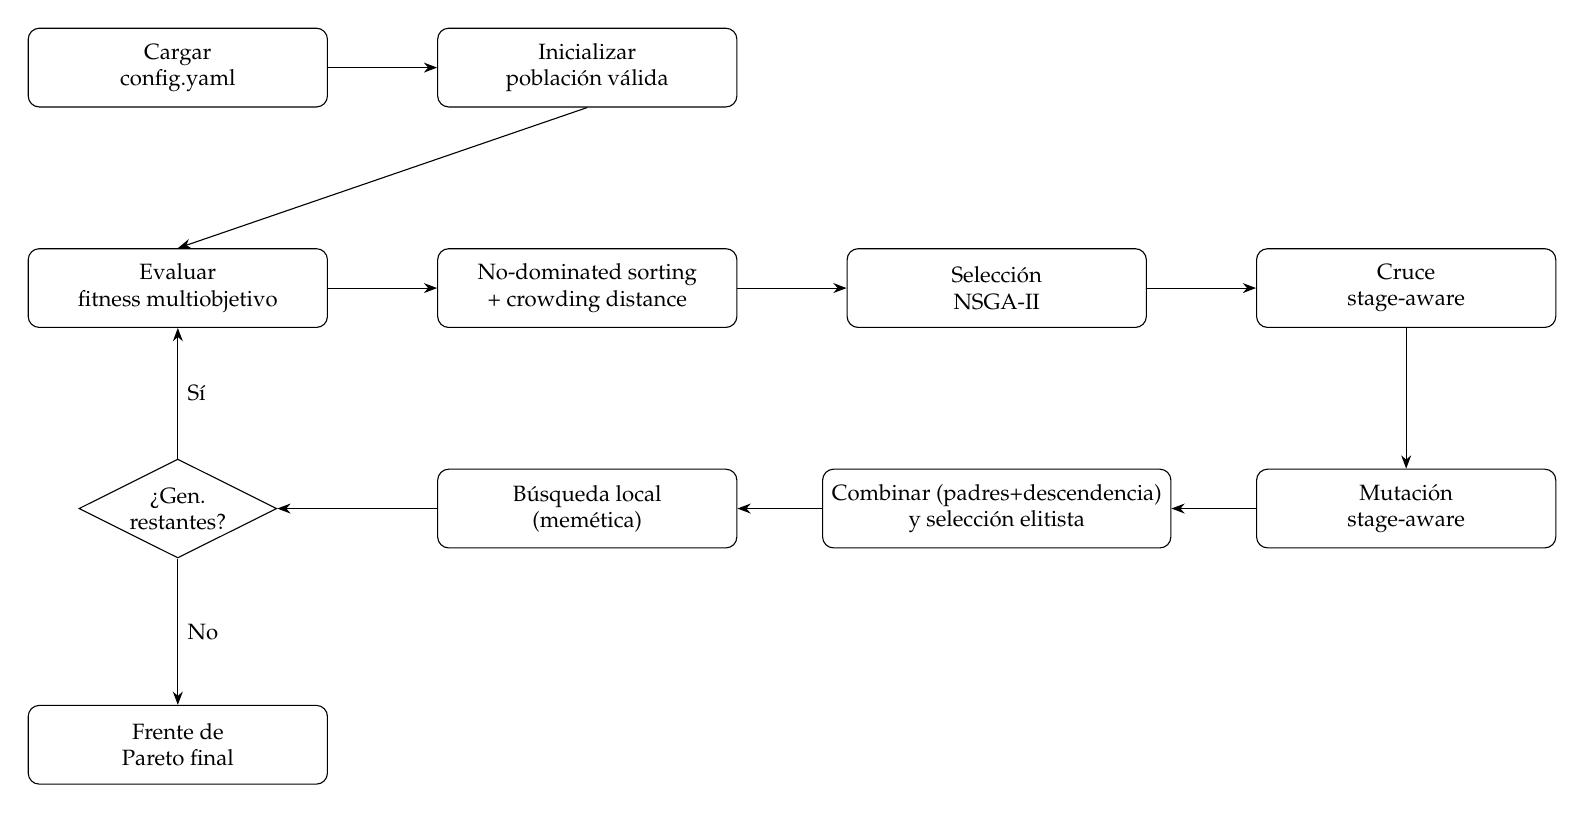
\begin{tikzpicture}[
    >=Stealth,
    proc/.style={rectangle, draw, rounded corners, align=center, minimum width=38mm, minimum height=10mm},
    decision/.style={diamond, draw, aspect=2, align=center, inner sep=1pt},
    small/.style={font=\footnotesize}
]
% Coordenadas base (4 niveles) en flujo serpiente (zig-zag)
% Nivel 1 (izq -> der): Cargar, Inicializar
\node[proc, small] (cfg) at (0,0) {Cargar\\config.yaml};
\node[proc, small] (pop) at (5.2,0) {Inicializar\\población válida};
% Nivel 2 (izq -> der): Evaluar, NDS+crowding, Selección, Cruce
\node[proc, small] (fit) at (0,-2.8) {Evaluar\\fitness multiobjetivo};
\node[proc, small] (nds) at (5.2,-2.8) {No-dominated sorting\\+ crowding distance};
\node[proc, small] (sel) at (10.4,-2.8) {Selección\\NSGA-II};
\node[proc, small] (cru) at (15.6,-2.8) {Cruce\\stage-aware};
% Nivel 3 (der -> izq): Mutación, Combinar+selección, Búsqueda local, ¿Gen.?
\node[proc, small] (mut) at (15.6,-5.6) {Mutación\\stage-aware};
\node[proc, small] (comb) at (10.4,-5.6) {Combinar (padres+descendencia)\\y selección elitista};
\node[proc, small] (loc) at (5.2,-5.6) {Búsqueda local\\(memética)};
\node[decision, small] (gen) at (0,-5.6) {¿Gen.\\restantes?};
% Nivel 4: Frente de Pareto (final)
\node[proc, small] (pareto) at (0,-8.6) {Frente de\\Pareto final};

% Conexiones principales en serpiente
\draw[->] (cfg.east) -- (pop.west);
\draw[->] (pop.south) -- (fit.north);           % baja al inicio de la fila 2 (izquierda)
\draw[->] (fit.east) -- (nds.west);
\draw[->] (nds.east) -- (sel.west);
\draw[->] (sel.east) -- (cru.west);
\draw[->] (cru.south) -- (mut.north);           % baja al inicio de la fila 3 (derecha)
\draw[->] (mut.west) -- (comb.east);
\draw[->] (comb.west) -- (loc.east);
\draw[->] (loc.west) -- (gen.east);
% Decisión
\draw[->] (gen.south) -- node[right, small]{No} (pareto.north);
\draw[->] (gen.north) -- node[midway, right, small]{Sí} (fit.south); % retorno recto a la parte inferior de evaluación
\end{tikzpicture}
}%
\caption{Pipeline del sistema: desde carga de configuración hasta obtención del frente de Pareto.}
\label{fig:pipeline}
\end{figure}


%\newpage
%$\ $
%\thispagestyle{empty} % para que no se numere esta pagina
\chapter{Resultados y Discusión}

\section{Resultados}
\subsection{Implementación en python}
La implementación de la función de fitness como se observa en la figura \ref{fitness_python} sigue el modelo visto en la metodología, considerando las condiciones del problema, así como ciertos incrementos los cuales fueron generados de forma aleatoria, por el código visto en la figura \ref{incrementos}, de esta forma los parámetros fijo utilizados como condiciones son los que se aprecian en la figura \ref{parametros}

\begin{figure}[H]
\centering
\includegraphics[width=0.9\textwidth]{Figures/apendice/implementaciones/incrementos.png}
\caption{Generación de incrementos}
\label{incrementos}
\end{figure}

\begin{figure}[H]
\centering
\includegraphics[width=0.75\textwidth]{Figures/apendice/implementaciones/parametros.png}
\caption{Generación de incrementos}
\label{parametros}
\end{figure}

Por otro lado, la implementación de la función de generación de la población inicial, vista en la figura \ref{poblacion}, mantuvo las condiciones iniciales y las señaladas en la metodología, al hacer uso de $set()$ y tener un conjunto de individuos existentes con los que comparar cada individuo generado es que se garantiza que cada individuo que ingrese a la población inicial sea único, sin embargo el fitness que estos puedan tener si puede llegar a coincidir.

\begin{figure}[H]
\centering
\includegraphics[width=0.7\textwidth]{Figures/apendice/implementaciones/población.png}
\caption{Generación de la población inicial}
\label{poblacion}
\end{figure}

Cada método de selección, cruza y mutación descritos en la metodología se logran implementar en su totalidad, añadiendo una condición. Posterior a la selección de padres, en caso se realice el cruzamiento, los dos individuos que se retornan de la función de cruzamiento para la siguiente generación son los que tengan el mejor fitness entre los 2 padres y 2 hijos, como se visualiza en la figura \ref{SEC_CRUZA_1} la cual es una sección de la implementación del cruzamiento mono-punto, de esta forma cada par de individuos elegidos siempre tendrán los mejores fitness posibles luego del proceso de selección-cruzamiento para pasar a la mutación.

\begin{figure}[H]
\centering
\includegraphics[width=0.8\textwidth]{Figures/apendice/implementaciones/seccion_cruza_1_punto.png}
\caption{Sección de codigo de cruzamiento en 1 punto}
\label{SEC_CRUZA_1}
\end{figure}

De esta forma es que el meta-algoritmo queda como se puede apreciar en la figura \ref{meta_alg}. El código fuente completo de la implementación, la data recopilada en cada ejecución y gráficos de cada modelo en sus diferentes iteraciones pueden encontrarse en el repositorio del proyecto \cite{link_trabajo} visitando el link del apéndice \ref{AppendC}.

\subsection{Mejor algoritmo elegido}

A partir de la data de las ejecuciones de los 120 AG, se tuvo como resultado lo apreciado en las figuras de apéndice \ref{AppendA}, esas figuras permiten ver como cada una de los 12 modelos de hiperparámetros categóricos se desempeña para cada una las 10 configuraciones de la figura \ref{conf_p_mod}, al aplicar los criterios de De Jong descritos en la metodología es que se descartan modelos los cuales tengan un promedio de promedios de makespan bastante elevado, como el modelo 1 visto en la figura \ref{mod1_graf} el cual tiene los promedio de promedios mas altos, como limite para un promedio de promedios se estableció un makespan de 1560 minutos

Adicionalmente al usar el criterio de robustez y ordenar los 120 AG posibles en base a sus desviaciones estándar de los \textit{promedio de makespan de las ultimas 60 generaciones} de cada ejecución, se tuvo como AG finalistas a un total de 10 AG, como se aprecia en la figura \ref{mej_10}.

A partir de los anterior y considerando los criterios de De Jong, el AG a seleccionar tuvo los siguientes hiperparámetros categóricos y numéricos:

Hiperparámetros categóricos:
\begin{itemize}
    \item Método de selección: Selección por ranking
    \item Método de cruzamiento: Cruce mono-punto
    \item Método de mutación: Mutación por intercambio de etapa
\end{itemize}

Hiperparámetros numéricos:
\begin{itemize}
    \item Tamaño de población: 240
    \item Probabilidad de cruzamiento: 57.485\%
    \item Probabilidad de mutación: 49.002\%
\end{itemize}

Esto debido a que al tener un promedio total de makespan menor al promedio de promedios de las ultimas 60 generaciones por ejecución, se puede apreciar que en esas ultimas 60 generaciones el algoritmo no convergió de manera apresurada, además de tener una desviación estándar baja, de 3.381 aproximadamente, es que este AG es el que ofrece un resultado mejor y más consistente a través de diversas ejecuciones.

\section{Discusión}
Los resultados previos contrastan con los vistos por Lopez, et al. \cite{Lop_et_al_2015}, dado que la variación de resutltados vista en este seminario es del 0.217\%, la cual es la variación que tendrá en base a la desviación estándar en relación con el promedio del makespan de las ultimas 60 generación por ejecución, esto indica que el AG desarrollado en este seminario es más robusto.

Al igual que en este seminario, Muñoz, et al. \cite{Mun_etal_2024} aborda el tema de la programación de maquinas en una linea de ensamblaje automotriz, con la diferencia que los autores trabajan 2 lineas de ensamblaje para poder operar 29 máquinas, sin embargo su AE utilizado tuvo 2 algoritmos de metaheuristicas, procedimiento de búsqueda adaptativa aleatoria voraz (GRASP) y el algoritmo genético de clave aleatoria sesgada (BRKGA), la diferencia principal es que los autores disponían del makespan optimo a alcanzar, sin embargo, en el presente seminario se busca tener un AG robusto que pueda competir de manera independiente de la cantidad de trabajos que requieran de una programación. De forma similar se explora otro camino de la aplicación de los AG basados en el modelo estándar de selección, cruza y mutación pero condicionando cada uno para acercarse lo más posible a la realidad.

Por otro lado los resultados hallados por Kraul \cite{KRAUL2025125624} en su solución para el problema de HFS, pero de 2 etapas, con el algoritmo genético logrando una brecha de desviación del 9.74\% y un tiempo de ejecución promedio de 9.81 segundos, por parte de este seminario el porcentaje de desviación fue del 0.217\%, pero con un tiempo de ejecución aproximado de 37 segundos aproximadamente. Si bien es casi 4 veces el tiempo de ejecución a comparación de los autores, el porcentaje de desviación es significativamente menor, por lo que es comparativamente mejor a nivel de robustez, esto también muestra una limitación del AG lo que muestra que aun queda aspectos por mejorar.

% [Sección de complejidad eliminada; movida al Capítulo 3]



%\newpage
%$\ $
%\thispagestyle{empty} % para que no se numere esta pagina
\chapter{Conclusiones y Trabajo Futuro}

\section{Conclusiones}

Este proyecto de tesis ha logrado establecer una base sólida para la implementación de algoritmos evolutivos multiobjetivo en la optimización de líneas de ensamblaje. A continuación se presentan las conclusiones principales del trabajo realizado hasta el momento:

\begin{itemize}

\item[•] El enfoque multiobjetivo implementado mediante NSGA-II y su variante memética representa una evolución significativa respecto a métodos monoobjetivo tradicionales. La formulación de tres objetivos simultáneos (makespan, balance de carga y consumo energético) permite capturar la complejidad real de los sistemas de manufactura, proporcionando al decisor múltiples soluciones Pareto-óptimas.

\item[•] La implementación del algoritmo NSGA-II con operadores especializados para problemas de programación en líneas de ensamblaje (cruce uniforme por etapa, mutaciones stage-aware) ha demostrado ser efectiva para explorar el espacio de soluciones manteniendo la validez de las configuraciones generadas. Los operadores desarrollados están específicamente adaptados a la estructura de etapas del problema, respetando las restricciones de máquinas disponibles por etapa.

\item[•] La adaptación del problema monoobjetivo original a un enfoque multiobjetivo con tres objetivos permite considerar simultáneamente aspectos de productividad, equidad operativa y sostenibilidad energética. Esta transformación enriquece el análisis y proporciona soluciones más completas para sistemas de manufactura modernos.

\item[•] El desarrollo de la función de fitness multiobjetivo que considera el desgaste de máquinas y procesos de enfriamiento añade realismo al modelo, permitiendo que el algoritmo opere bajo condiciones similares a entornos industriales reales.

\end{itemize}

\subsection{Estado Actual del Proyecto}

En la fase actual del proyecto, se ha completado la implementación de los algoritmos NSGA-II estándar y memético, junto con los operadores de cruce y mutación especializados. Asimismo, se ha desarrollado la función de evaluación multiobjetivo que considera los tres objetivos simultáneamente.

Los siguientes pasos del proyecto incluyen la realización de experimentos sistemáticos para determinar la configuración óptima de los algoritmos. Específicamente, se está próximo a ejecutar:

\begin{itemize}
    \item Experimentos de \textit{tunning multiobjetivo} para optimizar los hiperparámetros numéricos (tamaño de población, número de generaciones, probabilidades de cruce y mutación) considerando múltiples métricas de calidad del frente de Pareto.
    
    \item Experimentos de comparación de operadores para evaluar sistemáticamente las diferentes combinaciones de métodos de cruce y mutación, determinando cuáles proporcionan mejores resultados en términos de calidad, diversidad y convergencia del frente de Pareto.
    
    \item Análisis comparativo entre la versión estándar del NSGA-II y su variante memética para determinar en qué condiciones la búsqueda local aporta mejoras significativas.
\end{itemize}

Estos experimentos permitirán seleccionar la configuración más adecuada que se ajuste al problema específico, considerando criterios como robustez, replicabilidad y calidad de las soluciones obtenidas. Se espera que los resultados de estos experimentos proporcionen evidencia empírica sobre la efectividad del enfoque multiobjetivo propuesto para problemas de programación en líneas de ensamblaje.

\section{Trabajo Futuro}

Una vez completados los experimentos de tunning multiobjetivo y comparación de operadores, se plantean las siguientes líneas de trabajo futuro:

\subsection*{Análisis de Escalabilidad y Performance}
Se planea evaluar la escalabilidad del algoritmo implementado con diferentes tamaños de instancias del problema (número de pedidos, número de máquinas, etc.), analizando tanto el tiempo de ejecución como la calidad de las soluciones obtenidas. Este análisis permitirá identificar limitaciones y oportunidades de mejora.

%\afterpage{\blankpage}



\bibliography{main}
\bibliographystyle{unsrt}
\afterpage{\blankpage}

%\appendix
%% Appendix A

%\chapter{Gráficos de resultados}
%\label{AppendA} % For referencing this appendix elsewhere, use \ref{AppendixA}
%\Promedios de las 60 ultimas generaciones por cada modelo:
%\begin{figure}[H]
%\centering
%\includegraphics[width=1.0\textwidth]{Figures/apendice/prom_modelos/graf_tiempo_mod_1.png}
%\caption{Modelo 1, 10 configuraciones}
%\label{mod1_graf}
%\end{figure}

%\begin{figure}[H]
%\centering
%\includegraphics[width=1.0\textwidth]{Figures/apendice/prom_modelos/graf_tiempo_mod_2.png}
%\caption{Modelo 2, 10 configuraciones}
%\label{mod2_graf}
%\end{figure}

%\begin{figure}[H]
%\centering
%\includegraphics[width=1.0\textwidth]{Figures/apendice/prom_modelos/graf_tiempo_mod_3.png}
%\caption{Modelo 3, 10 configuraciones}
%\label{mod3_graf}
%\end{figure}

%\begin{figure}[H]
%\centering
%\includegraphics[width=1.0\textwidth]{Figures/apendice/prom_modelos/graf_tiempo_mod_4.png}
%\caption{Modelo 4, 10 configuraciones}
%\label{mod4_graf}
%\end{figure}

%\begin{figure}[H]
%\centering
%\includegraphics[width=1.0\textwidth]{Figures/apendice/prom_modelos/graf_tiempo_mod_5.png}
%\caption{Modelo 5, 10 configuraciones}
%\label{mod5_graf}
%\end{figure}

%\begin{figure}[H]
%\centering
%\includegraphics[width=1.0\textwidth]{Figures/apendice/prom_modelos/graf_tiempo_mod_6.png}
%\caption{Modelo 6, 10 configuraciones}
%\label{mod6_graf}
%\end{figure}

%\begin{figure}[H]
%\centering
%\includegraphics[width=1.0\textwidth]{Figures/apendice/prom_modelos/graf_tiempo_mod_7.png}
%\caption{Modelo 7, 10 configuraciones}
%\label{mod7_graf}
%\end{figure}

%\begin{figure}[H]
%\centering
%\includegraphics[width=1.0\textwidth]{Figures/apendice/prom_modelos/graf_tiempo_mod_8.png}
%\caption{Modelo 8, 10 configuraciones}
%\label{mod8_graf}
%\end{figure}

%\begin{figure}[H]
%\centering
%\includegraphics[width=1.0\textwidth]{Figures/apendice/prom_modelos/graf_tiempo_mod_9.png}
%\caption{Modelo 9, 10 configuraciones}
%\label{mod9_graf}
%\end{figure}

%\begin{figure}[H]
%\centering
%\includegraphics[width=1.0\textwidth]{Figures/apendice/prom_modelos/graf_tiempo_mod_10.png}
%\caption{Modelo 10, 10 configuraciones}
%\label{mod10_graf}
%\end{figure}

%\begin{figure}[H]
%\centering
%\includegraphics[width=1.0\textwidth]{Figures/apendice/prom_modelos/graf_tiempo_mod_11.png}
%\caption{Modelo 11, 10 configuraciones}
%\label{mod11_graf}
%\end{figure}

%\begin{figure}[H]
%\centering
%\includegraphics[width=1.0\textwidth]{Figures/apendice/prom_modelos/graf_tiempo_mod_12.png}
%\caption{Modelo 12, 10 configuraciones}
%\label{mod12_graf}
%\end{figure}
%\chapter{Tablas de Datos Complementarios} % Main appendix title

%\label{AppendB}

%Configuraciones por modelo:

%\begin{figure}[H]
%\centering
%\includegraphics[width=0.9\textwidth]{Figures/Criterios/configuraciones.png}
%\caption{Configuraciones para cada modelo}
%\label{conf_p_mod}
%\end{figure}

%Mejores diez algoritmos seleccionados:

%\begin{figure}[H]
%\centering
%\includegraphics[width=1.0\textwidth]{Figures/Criterios/mejores_10.png}
%\caption{Mejores 10 algoritmos genéticos seleccionados}
%\label{mej_10}
%\end{figure}
%############# Apendice C %#############
\chapter{Código Fuente del Algoritmo} % Main appendix title
\label{AppendA}

Repositorio del proyecto:

\begin{verbatim}
    https://github.com/luis1310/HFS-T2/tree/tesis3-dev
\end{verbatim}

%Implementación de función de fitness:
%\begin{figure}[H]
%\centering
%\includegraphics[width=0.9\textwidth]{Figures/apendice/implementaciones/fitness_python.png}
%\caption{Implementación de la función de fitness}
%\label{fitness_python}
%\end{figure}

%Implementación de Meta-Algoritmo:
%\begin{figure}[H]
%\centering
%\includegraphics[width=0.9\textwidth]{Figures/apendice/implementaciones/Meta_algoritmo.png}
%\caption{Implementación del Meta-Algoritmo en python}
%\label{meta_alg}
%\end{figure}











\end{document}